\chapter{Material equations} \label{cha:material_equations}

\section{Introduction}

In \secref{sec:geometry_and_physics}, we have described how to
associate physical quantities to the geometrical elements of the
computational mesh. We have also pointed out that Maxwell equations are
purely topological relations, exactly satisfied by the degrees of
freedom chosen, while errors, unavoidably introduced by the
discretization process, are caused only by the non-perfect modeling of
material equations. The resulting material matrices, also called \emph{mass
matrices} in Finite Elements context and \emph{discrete Hodge
operators} in differential geometry, greatly affects the stability and
the accuracy of time- and frequency-domain algorithms
\cite{schuhmann_whitney,schuhmann_stability}.

In the next sections we'll describe how to build the material
matrices, given a primal mesh, for different dual meshes: in
particular, for the Vorono\"i, Poincar\'e and barycentric dual grids.

\section{Vorono\"i Dual Mesh} \label{sec:voronoi}

As described in \secref{sec:dual_mesh}, given a primal simplicial Delaunay
mesh, its Vorono\"i dual mesh is built connecting the spherocenters of
the primal cells. Some properties hold:
\begin{itemize}
\item
  dual edges are orthogonal to primal faces;
\item
  primal edges are orthogonal to dual faces;
\item
  dual volumes are the loci of nearest points to the corresponding
  primal point.
\end{itemize}

These properties represent, as we'll see later, an advantage in modeling
Maxwell equations, but they represent tough geometrical
constrains that meshing software must satisfy in order to generate
proper meshes \cite{triangle}.

Consider a Delaunay primal mesh and its Vorono\"i dual mesh and let:
\begin{align} \label{eqn:voronoi_dof}
e_i & = \DotProd{\E}{\Versor{p}_i} \Line{e}_i \\
h_i & = \DotProd{\H}{\Versor{s}_i} \DualLine{e}_i \\
b_i & = \DotProd{\B}{\Versor{s}_i} \Surface{f}_i \\
d_i & = \DotProd{\D}{\Versor{p}_i} \DualSurface{f}_i,
\end{align}
where $\Versor{p}_i$ ($\Versor{s}_i$) is the primal (dual) edge
versor, be the realization of the mapping shown in
\eqref{eqn:dof}. The integral is not necessary because edges are
considered straight and $\E$ is considered piecewise constant along each
edge. From the definition of Vorono\"i dual mesh, $\Versor{p}_i$ is
orthogonal to $\Versor{s}_i$. See \figref{fig:voronoi}.

\begin{figure}[htbp]
  \begin{center}
    \subfigure[The dual edge $\DualLine{e}_i$ is orthogonal to
      the primal face $\Surface{f}_i$.]{\resizebox{!}{5cm}{\input{pics/voronoi_primal.pdf_t}}}
    \subfigure[The edge $\Line{e}_i$ is orthogonal to
      the dual face $\DualSurface{f}_i$]{\resizebox{!}{5cm}{\input{pics/voronoi_dual.pdf_t}}}
  \end{center}
  \caption{Vorono\"i dual mesh.}
  \label{fig:voronoi}
\end{figure}

Maxwell equations read:
\begin{equation} \label{eqn:voronoi_maxwell} \begin{cases}
    \Disc{b_i}{}{n+1/2} & = \Disc{b_i}{}{n-1/2} - \deltat \sum_{j \in
    \Set{B}_{\Surface{f}_i}} \Disc{e_j}{}{n} \\
    \Disc{d_i}{}{n+1} & = \Disc{d_i}{}{n-1} + \deltat \sum_{j \in
    \Set{B}_{\DualSurface{f}_i}} \Disc{h_j}{}{n+1/2}.
  \end{cases} \end{equation}

$\Set{B}_{\Surface{f}_i}$ is the set of the indices that identifies the border
edges of the primal face $\Surface{f}_i$:
\begin{equation*}
  \Set{B}_{\Surface{f}_i} = \left\{ j\ :\ \Line{e}_j \in \partial \Surface{f}_i \right\}
\end{equation*}
where $\partial \Surface{f}$ denotes the boundary of the face $\Surface{f}$, and
$\Set{B}_{\DualSurface{f}_i}$ is the set of the indices that identifies the border
edges of the dual face $\DualSurface{f}_i$:
\begin{equation*}
  \Set{B}_{\DualSurface{f}_i} = \left\{ j\ :\ \DualLine{e}_j \in \partial \DualSurface{f}_i \right\}
\end{equation*}

Thank to the properties of Vorono\"i meshes, the constitutive
equations are straightforward. From \eqref{eqn:voronoi_dof}, consider
the $i^{th}$ primal face, and the corresponding $i^{th}$ (orthogonal) dual edge; we
can write:
\begin{equation} \label{eqn:voronoi_constitutive_magnetic}
  h_i = \frac{\Measure{\DualLine{e}_i}}{\Measure{\Surface{f}_i} \mu_i} b_i
\end{equation}
where $\mu_i$ is the magnetic permeability associated to the primal
face $\Surface{f}_i$: it is supposed piecewise constant on
it. $\Measure{\DualLine{e}}$ and $\Measure{\DualSurface{f}}$ are the
measures of the dual edge $\DualLine{e}$ and the dual face
$\DualSurface{f}$, respectively; as we can note, material matrices
require a metric to be defined \cite{bossavit_computational}: they are
not purely topological relations! We have chosen to use the classical
Euclidean norm, as measure.

The other constitutive equation, for the $i^{th}$ primal edge and the
$i^{th}$ dual face, reads:
\begin{equation} \label{eqn:voronoi_constitutive_electric}
  e_i = \frac{\Measure{\Line{e}_i}}{\Measure{\DualSurface{f}_i} \epsilon_i} d_i
\end{equation}
where $\epsilon_i$ is the electric permeability associated to the dual
face $\DualSurface{f}_i$: it is supposed piecewise constant on it.

Note that the value of $h_i$ ($e_i$) only depends on the value of
$b_i$ ($d_i$) on the corresponding (dual) face. Rewriting
\eqref{eqn:voronoi_constitutive_magnetic} and
\eqref{eqn:voronoi_constitutive_electric} in matrix form, we have:
\begin{align*}
  \Array{h} & = \Prod{\Matrix{M}_\mu}{\Array{b}} \\
  \Array{e} & = \Prod{\Matrix{M}_\epsilon}{\Array{d}} ,
\end{align*}
where $\Array{h}$ and $\Array{b}$ are the arrays of all the $h_i$ and
$b_i$ in \eqref{eqn:voronoi_maxwell} and $\Matrix{M}_\epsilon$ and
$\Matrix{M}_\mu$ are square diagonal matrices whose dimensions are the number
of dual and primal faces, respectively:
\begin{align*}
  \Matrix{M}_\mu \in \nf \times \nf && \Matrix{M}_\epsilon \in \ndf \times \ndf .
\end{align*}

\section{Poincar\'e Dual Mesh} \label{sec:poicare}

Given a primal triangular mesh, the Poincar\'e dual mesh is built
connecting the barycenters of the primal volumes. Comparing to the
Vorono\"i dual mesh, we can note:
\begin{enumerate}
\item
  the dual points are always inside the primal volumes: this makes the
  scheme more stable in the time-domain;
\item
  the dual edges are not orthogonal to the primal faces and the primal
  edges are not orthogonal to the dual faces: this makes the
  constitutive relations more complicated to implement.
\end{enumerate}

Consider a 2D triangular primal mesh, as in \figref{fig:poincare} and
let's limit to the study of the TE polarization\footnote{for the TM
polarization, the Duality Theorem can be applied
\cite{someda_electromagnetic}; the extension to the 3D case is
straightforward, too.}: let $E_z$ and $D_z$ be associated to the nodes
of the primal grid and $\H_t$ and $B_t$ to the edges of the dual grid.

\begin{figure}[htbp]
  \begin{center}
    \resizebox{4cm}{!}{\input{pics/poincare.pdf_t}}
  \end{center}
  \caption{Poincar\'e dual mesh: primal (dual) edges are not
    orthogonal to dual (primal) faces. In two-dimensional meshes, some
    primal faces are actually edges. In red, identified with $j$, are
    the primal faces (actually edges) sharing a common vertical primal
    edge (actually a point) with the primal face (actually an edge)
    $i$.}
  \label{fig:poincare}
\end{figure}

Let:
\begin{align} \label{eqn:dof_poincare}
e_i & = \DotProd{\E}{\Versor{p}_i} \ell_i \\
h_i & = \DotProd{\H}{\Versor{s}_i} \Dual{\ell}_i \\
b_i & = \DotProd{\B}{\Versor{n}_{p_i}} A_i \\
d_i & = \DotProd{\D}{\Versor{n}_{s_i}} \Dual{A}_i
\end{align}
where $\Versor{p}_i$ ($\Versor{s}_i$) is the primal (dual) edge
versor and $\Versor{n}_{p_i}$ ($\Versor{n}_{s_i}$) is the versor
orthogonal to the primal (dual) face. As noted before,
$\Versor{n}_{p_i}$ is not parallel to $\Versor{s}_i$ and
$\Versor{n}_{s_i}$ is not parallel to $\Versor{p}_i$ as in
Vorono\"i dual grids.

Maxwell equations, being topological relations, are the same as for
the Vorono\"i dual mesh, in \eqref{eqn:voronoi_maxwell}.

Constitutive equations are more complicated because $\H_t \nparallel
\B_t$. For the electric constitutive equation,
\eqref{eqn:voronoi_constitutive_electric}, valid in the Vorono\"i
case, holds: this is because we are dealing now only with the TE case,
for which the electric field component $E_z$ is orthogonal to dual
faces (which lie on the $xy$ plane). For the magnetic constitutive
equation, recall that we have to write:
\begin{equation*}
  \Array{h} = \Prod{\Matrix{M}_\mu}{\Array{b}} ,
\end{equation*}
where $\Array{h}$ and $\Array{b}$ are the arrays of all the $h_i$ and
$b_i$ in \eqref{eqn:voronoi_maxwell} and $\Matrix{M}_\mu$ is a square
matrix whose dimension is the number of dual edges (or primal faces).

This can be done in three steps \cite{taflove_advances}.
\begin{enumerate}
\item
  Consider the primal face $\Surface{f}_i$ and all the faces
  $\Surface{f}_j$ sharing with it one edge, like in
  \figref{fig:poincare}. Write $\B_j$, the magnetic field on the face
  $\Surface{f}_j$, as a linear combination of $b_i$ and $b_j$,
  magnetic fluxes through $\Surface{f}_i$ and $\Surface{f}_j$:
  \begin{equation*} \begin{cases}
      \DotProd{\B_j}{\Vector{N}_{p_i}} & =
      \DotProd{\B}{\Vector{N}_{p_i}} = b_i \\
      \DotProd{\B_j}{\Vector{N}_{p_j}} & =
      \DotProd{\B}{\Vector{N}_{p_j}} = b_j .
  \end{cases} \end{equation*}
  where $\Vector{N}_{p_i} = \Versor{n}_{p_i} \Measure{\Surface{f}_i}$
  and the same for $\Vector{N}_{p_j}$. This comes from flux conservation.
  
  The right-hand sides are known from Faraday equation (the first
  in \eqref{eqn:voronoi_maxwell}), so we can calculate $\B_j$:
  \begin{align*}
    \B_j = \Prod{\Matrix{N}^{-1}}{\begin{bmatrix} b_i \\ b_j \end{bmatrix}}
    && \text{where} && \Matrix{N} = \begin{bmatrix} N^x_{p_i}
    & N^y_{p_i} \\ N^x_{p_j} & N^y_{p_j} \end{bmatrix} .
  \end{align*}
\item
  Write $\B$ as a linear combination of $\B_j$:
  \begin{equation*}
    \B_i = \frac{1}{W} \sum_j w_j \B_j ,
  \end{equation*}
  where $W = \sum_j w_j$ and $w_j = \Norm{\DotProd{\Versor{z}}{\left(
  \CrossProd{\Vector{N}_{p_i}}{\Vector{N}_{p_j}} \right)}}$ are
  weighting coefficients whose value is twice the area of the triangle
  identified by the edges $i$ and $j$.
\item
  Finally, compute $\H$ from the continuum constitutive relation $\H = \mu^{-1} \B$ and
  then $h_i$, from \eqref{eqn:poincare_dof}:
  \begin{equation} \label{eqn:poincare_constitutive_magnetic} \begin{split}
    h_i & = \DotProd{\H}{\Versor{s}_i} \Measure{\DualLine{e}_i} \\
    & = H_x \Measure{\DualLine{e}_i} \cos\beta + H_y \Measure{\DualLine{e}_i} \sin\beta \\
    & = \mu_x^{-1} B_x \Measure{\DualLine{e}_i} \cos\beta +
    \mu_y^{-1} B_y \Measure{\DualLine{e}_i} \sin\beta \\
    & = \frac{1}{W} \sum_j w_j \left[ \mu_x^{-1} B_x \Measure{\DualLine{e}_i}
    \cos\beta + \mu_y^{-1} B_y \Measure{\DualLine{e}_i}
    \sin\beta \right] \\
    & = \frac{1}{W} \sum_j w_j \left[ \mu_x^{-1} \Measure{\DualLine{e}_i}
    \cos\beta \left( k_{11} b_i + k_{12} b_j \right) +
    \mu_y^{-1} \Measure{\DualLine{e}_i} \sin\beta \left( k_{21} b_i +
    k_{22} b_j \right) \right] \\
    & = \frac{\Measure{\DualLine{e}_i}}{W} \sum_j w_j \left[ \left( \mu_x^{-1} k_{11}
    \cos\beta + \mu_y^{-1} k_{21} \sin\beta
    \right) b_i + \left( \mu_y^{-1} k_{12}
    \cos\beta + \mu_y^{-1} k_{22} \sin\beta
    \right) b_j \right]
  \end{split} \end{equation}
  where $\beta$ is the angle between the dual edge $\DualLine{e}_i$ and
  the $x$-axis and $\Matrix{K} = \bigl[ \begin{smallmatrix}
  k_{11}&k_{12}\\k_{21}&k_{22} \end{smallmatrix} \bigr] =
  \Matrix{N}^{-1}$.
  
  In matricial form, \eqref{eqn:poincare_constitutive_magnetic} reads:
  \begin{equation*}
    \Array{h} = \Prod{\Matrix{M}_\mu}{\Array{b}} ,
  \end{equation*}
  where
  \begin{equation} \label{eqn:constitutive_poincare}
    \Matrix{M}_\mu = \begin{bmatrix}
      {\Matrix{M}_\mu}_{ij}
    \end{bmatrix} = \begin{cases}
      \frac{\Measure{\DualLine{e}}}{W} \sum_j w_j 
    \left( \mu_x^{-1} k_{11} \cos\beta + \mu_y^{-1} k_{21} \sin\beta
    \right) & \text{for $i = j$} \\
      \frac{\Measure{\DualLine{e}}}{W} w_j 
    \left( \mu_x^{-1} k_{12} \cos\beta + \mu_y^{-1} k_{22} \sin\beta
    \right) & \text{for $i \neq j$} \\
    \end{cases}
  \end{equation}
\end{enumerate}

It is worth noting that:
\begin{itemize}
\item
  these three steps are fully explicit, i.e. we
  don't ever need to solve a linear system to compute the unknowns we
  need;
\item
  the final matrix $\Matrix{M}_\mu$ is not diagonal, as
  explicitly stated in \eqref{eqn:constitutive_poincare}: this is not
  a problem, neither in the time- nor in the frequency-domain;
\item
  \eqref{eqn:poincare_constitutive_magnetic} is valid also for
  anisotropic materials: just use a tensor $\mu = \left[
  \begin{smallmatrix} \mu_{xx} & \mu_{xy} \\ \mu_{yx} & \mu_{yy}
  \end{smallmatrix} \right]$. Note also that dealing with an
  anisotropic material is equivalent in introducing a local change of
  metric. In fact, for the simple case of a coordinate system oriented
  with the crystallographic axis of the anisotropic
  material\footnote{If not, a simple rotation of the reference axis
  can bring us to this condition}:
  \begin{equation*} \begin{split}
    h_i & = \Prod{\left( \mu^{-1} \B \right)}{\Versor{s}_i} \Measure{\DualLine{e}_i} \\
        & = \left( \mu_x^{-1} {s_i}_x B_x + \mu_y^{-1} {s_i}_y B_y \right) \Measure{\DualLine{e}_i} \\
        & = \Prod{\B}{\Vector{s}'_i} \Measure{\DualLine{e}_i}
  \end{split} \end{equation*}
  where $\Vector{s}'_i = \left( \mu_x^{-1} {s_i}_x, \mu_y^{-1}
  {s_i}_y \right)$. The metric, as said before, is needed when dealing
  with the material equations.
\end{itemize}

\subsection{Barycentric Dual Mesh} \label{sec:barycentric}

Given a triangular primal mesh, its barycentric dual is made of:
\begin{itemize}
\item
  dual points that are the barycenters of the primal volumes;
\item
  dual edges that are piece-lines made by two straight lines whose
  contact point is the barycenter of the corresponding primal face,
  and connect the dual points;
\item
  dual surfaces having as a border the dual lines surrounding the
  corresponding primal edge.
\end{itemize}

\begin{figure}[htbp]
  \begin{center}
    \resizebox{4cm}{!}{\input{pics/barycentric.pdf_t}}
  \end{center}
  \caption{Barycentric dual mesh: dual edges are piece-lines to
  connect barycenters of adjacent primal cells.}
  \label{fig:barycentric}
\end{figure}

Since primal and dual meshes are not orthogonal, as in the Poincar\'e
mesh, the constitutive equation requires a similar math to be worked
out. The advantage of this mesh is its superior stability and the
possibility to use any kind of triangular grid, not only a Delaunay
one \cite{marrone_computational}.

Consider a 2D TE case: the degrees of freedom are as in
\eqref{eqn:dof_poincare}. Consider the figure \OKKIO{figure 11 di
  marrone computational}, and divide the primal volume, as shown, in 6
\emph{micro-cells}. For each micro-cell, we can write:
\begin{align}
  \begin{bmatrix} \Phi_{1U''} \\ \Phi_{2U'} \end{bmatrix} = \Prod{
  \begin{bmatrix} S_{1U_x''} & S_{1U_y''} \\ S_{2U_y'} & S_{2U_y'}
  \end{bmatrix}}{
  \begin{bmatrix} B_x \\ B_y \end{bmatrix}}
\end{align}
where $\Phi$ is the magnetic flux through the primal face $S$, and
$\Vector{S}_{1U}$ is the vector normal to the primal face $1U$, whose
modulus is equal the area of the face. Something similar holds for the
$\H$ field:
\begin{align}
  \begin{bmatrix} F_{1U''} \\ F_{2U'} \end{bmatrix} = \Prod{
  \begin{bmatrix} \Dual{\ell}_{1U_x''} & \Dual{\ell}_{1U_y''} \\
    \Dual{\ell}_{2U_y'} & \Dual{\ell}_{2U_y'} \end{bmatrix}}{
  \begin{bmatrix} H_x \\ H_y \end{bmatrix}}
\end{align}
where $F$ is the circuitation of $\H$ along the dual line
$\Dual{\ell}$.

We can combine the two equations and the material equation $\B = \mu
\H$, to obtain:
\begin{align} \label{eqn:constitutive_barycentric_microcell}
  \begin{bmatrix} \Phi_{1U''} \\ \Phi_{2U'} \end{bmatrix} = \Prod{
  \underbrace{
  \begin{bmatrix} S_{1U_x''} & S_{1U_y''} \\ S_{2U_y'} & S_{2U_y'}
  \end{bmatrix}
  \mu
  \begin{bmatrix} \Dual{\ell}_{1U_x''} & \Dual{\ell}_{1U_y''} \\
    \Dual{\ell}_{2U_y'} & \Dual{\ell}_{2U_y'} \end{bmatrix}^{-1}
  }_{\Matrix{M}_\mu}}{
  \begin{bmatrix} F_{1U''} \\ F_{2U'} \end{bmatrix}}
\end{align}
This constitutive equation holds for the each micro-cell considered. We
can write 6 equations like this, one for each micro-cell in which the
primal volume is divided. Finally, we connect each other by continuity
condition, to get the final constitutive equation. For the continuity
of the $\H$ tangential component, we have:
\begin{align}
  F_{1U}' & = F_{1L}' & F_{1U}'' & = F_{1L}'' \\
  F_{2U}' & = F_{2L}' & F_{2U}'' & = F_{2L}'' \\
  F_{3U}' & = F_{3L}' & F_{3U}'' & = F_{3L}''
\end{align}
For the additivity of the flux of $\B$, i.e. the conservation of the
normal component of $\B$, we have:
\begin{align}
  \Phi_{1U}' + \Phi_{1U}' & = \Phi_{1}' & \Phi_{1U}'' + \Phi_{1U}'' & = \Phi_{1}'' \\
  \Phi_{2U}' + \Phi_{2U}' & = \Phi_{2}' & \Phi_{2U}'' + \Phi_{2U}'' & = \Phi_{2}'' \\
  \Phi_{3U}' + \Phi_{3U}' & = \Phi_{3}' & \Phi_{3U}'' + \Phi_{3U}'' & = \Phi_{3}''
\end{align}
Again, imposing the continuity of the $\H$ field:
\begin{align}
  F_1' & = F_1'' \\
  F_2' & = F_2'' \\
  F_3' & = F_3''
\end{align}
and the additivity of the flux of $\B$:
\begin{align}
  \Phi_1' + \Phi_1'' & = \Phi_1 \\
  \Phi_2' + \Phi_2'' & = \Phi_2 \\
  \Phi_3' + \Phi_3'' & = \Phi_3
\end{align}
This leads us to write the constitutive equation for the primal cell:
\begin{equation} \label{eqn:constitutive_barycentric}
  \begin{bmatrix} \Phi_1 \\ \Phi_2 \\ \Phi_3 \end{bmatrix} = \Prod{
  \underbrace{
    \begin{bmatrix}
      {M_\mu^a}_{11} & {M_\mu^a}_{12} & 0 \\
      {M_\mu^a}_{21} & {M_\mu^a}_{22} & 0 \\
      0 & 0 & 0 \\
    \end{bmatrix} +
    \begin{bmatrix}
      0 & 0 & 0 \\
      0 & {M_\mu^b}_{11} & {M_\mu^b}_{12} \\
      0 & {M_\mu^b}_{21} & {M_\mu^b}_{22}
    \end{bmatrix} +
    \begin{bmatrix}
      {M_\mu^c}_{22} & 0 & {M_\mu^c}_{21} \\
      0 & 0 & 0 \\
      {M_\mu^c}_{12} & 0 & {M_\mu^c}_{11}
    \end{bmatrix}
    }_{\Matrix{M}_\mu}}{
  \begin{bmatrix} F_1 \\ F_2 \\ F_3 \end{bmatrix}}
\end{equation}

On a perfectly dual way, the electric constitutive equation can be
written.

Note that anisotropy is readily implemented considering a tensor $\mu
= \left[ \begin{smallmatrix} \mu_{xx} & \mu_{xy} \\ \mu_{yx} &
  \mu_{yy} \end{smallmatrix} \right]$ in
\eqref{eqn:constitutive_barycentric_microcell}.

\subsection{Two dimensional extrude grids}

It is obtained by extrusion along the third dimension of a
two-dimensional grid. Good for planar structures.

\subsection{Particular material equations} \label{sec:particular_material_equations}

In the previous subsections the conventional material equations have
been discretized. We'll show now how more complex materials can be
modeled with the present method.

\subsubsection{Anisotropic materials}

\OKKIO{mettere qui i materiali anisotropi -- local change of metric}

\subsubsection{Ohm losses}

Equation \eqref{eqn:maxwell_time_domain} is missing the description of
the Ohm losses. It can be easily included, as follows:
\begin{equation*} \begin{cases}
  \Prod{\Transpose{\Matrix{R}}}{\Array{h}} = \partial_t \Array{d} + \Array{j} + \Matrix{\sigma_e} \Array{e} \\
  \Prod{\Matrix{R}}{\Array{e}} = -\partial_t \Array{b} + \Array{m} - \Matrix{\sigma_m} \Array{h}
\end{cases} \end{equation*}
According to the association of the degrees of freedom to the
geometrical elements of the mesh, supposing that the electric field
associated to a primal edge and the conductibility are uniform over the
corresponding dual face, we can easily build the matrices
$\Matrix{\sigma_e}$ and $\Matrix{\sigma_m}$ as the material matrices,
with the procedures described above, depending on the particular dual
grid chosen. The only problem arises in the time domain: in fact, the
matrix/operator $\Matrix{\sigma_e}$ ($\Matrix{\sigma_m}$) must link a
physical quantity defined on the primal instants (the electric field)
with one defined on the dual instants (the magnetic field). Hence, it
must be estimated by some means of time approximation. The easiest way
to do it, which keeps the algorithm stable, is to approximate the
electric field at the time-step $n+1/2$ as the mean value of the
instants before and after it:
\begin{equation*}
  \Disc{\Array{e}}{}{n+1/2} \simeq \frac{\Disc{\Array{e}}{}{n} + \Disc{\Array{e}}{}{n+1}}{2}
\end{equation*}
With this choice, \eqref{eqn:maxwell_time_domain} only involve fields
defined in the \emph{proper} time instants, and the algorithm is
stable (and second order accurate in the time derivative).

The same reasoning holds for the magnetic conductivity
$\Matrix{\sigma_m}$\footnote{Even if the magnetic conductivity can
  appear a useless physical quantity, it is not, because it is used in
  the modelling of PML losses}.

It should be clear that this problem only arises in the
time-domain. In the frequency domain, the easiest way to deal with Ohm
losses is to accept a complex value for the electric and magnetic
permeabilities. In formulas:
\begin{equation*}
    \begin{cases}
      \Rot{\H} = -\imath \omega \epsilon \E + \sigma_e \E \\
      \Rot{\E} = \imath \omega \mu \H + \sigma_m \H \\
    \end{cases}
    \Longrightarrow
    \begin{cases}
      \Rot{\H} = -\imath \omega \bar{\epsilon} \E \\
      \Rot{\E} = \imath \omega \bar{\mu} \H \\
    \end{cases}
\end{equation*}
where $\bar{\epsilon} = \epsilon + \imath \frac{\sigma_e}{\omega}$ and
$\bar{\mu} = \mu + \imath \frac{\sigma_m}{\omega}$. Obviously, also
the material matrices $\Matrix{M}_\epsilon$ and $\Matrix{M}_\mu$ will
be complex.

As a first approximation, we can disregard this problem, even in the
time-domain, and write: \OKKIO{controllare!!!}
\begin{equation*} \begin{cases}
    \frac{\Disc{\Array{b}}{}{n+1} - \Disc{\Array{b}}{}{n}}{\deltat} = -
    \Prod{\Matrix{R}}{\Disc{\Array{e}}{}{n+1/2}} -
    \Prod{\Matrix{\Omega}_{MN}}{\Disc{\Array{h}}{}{n-1}} \\
    \frac{\Disc{\Array{d}}{}{n+1/2} - \Disc{\Array{d}}{}{n-1/2}}{\deltat} = 
    \Prod{\Transpose{\Matrix{R}}}{\Disc{\Array{e}}{}{n+1/2}} -
    \Prod{\Matrix{\Omega}_{EN}}{\Disc{\Array{e}}{}{n-1/2}}
\end{cases} \end{equation*}
For later convenience, let $\Matrix{P}_m =
\Prod{\Matrix{M}_\mu}{\Matrix{\Omega}_{MN}}$ and $\Matrix{P}_e =
\Prod{\Matrix{M}_\epsilon}{\Matrix{\Omega}_{EN}}$.

$\Matrix{\Omega}_{MN}$ and $\Matrix{\Omega}_{EN}$ can be built
following the same procedure used for the material matrices.

\subsubsection{U-PML} \label{sec:pml}

PML are used to model infinite materials, i.e. to model the radiation
of light as if the boundaries of the computational domain were at
infinite distance from the source. There are mainly two formulations
to model the PMLs:
\begin{description}
\item[coordinate stretching]: in which a local change of metric is
  introduced where attenuation is needed, so that any plane wave
  impinging at the interface undergoes no reflection, but
  exponentially decays at zero;
\item[Uniaxial PML]: in which an anisotropic lossy material, but fully
  Maxwellian, is defined, with the property of absorbing, without
  reflections, any plane wave impinging to it.
\end{description}

Even if both the formulations have been successfully implemented in
many algorithm, we have decided to implement the second. The main
reason is that the U-PML are a fully Maxwellian medium, while the
medium in one is not: Maxwell's equations hold in the U-PMLs, but not
in the coordinate stretched system and new equation must be
implemented\footnote{In particular, Gauss equation fails to
  hold: at the interface between two different media inside the PMLs,
  the normal components of both $\E$ and $\D$ are continuous, instead
  of just $\D$. The same is valid for $\H$ and $\B$.}. Having a scheme
of degrees of freedom and geometrical elements fully functional to
solve Maxwell's equations it seems a waste of time to introduce a new
one only where PMLs are needed: laziness is a good quality for
scientists and programmers.

Uniaxial PMLs are an anisotropic lossy medium. Maxwell's equations in
this medium read:
\begin{equation*} \begin{cases}
    \Rot{\E} = -\imath \omega \Tensor{\mu} \H \\
    \Rot{\H} = \imath \omega \Tensor{\epsilon} \E + \J \\
\end{cases} \end{equation*}
where $\Tensor{\mu}$ and $\Tensor{\epsilon}$ are tensors defined as:
\begin{align*}
  \Tensor{\mu} & = \Prod{\mu}{\Tensor{s}} \\
  \Tensor{\epsilon} & = \Prod{\epsilon}{\Tensor{s}}
\intertext{and}
  \Tensor{s} & = \Prod{\Tensor{s}_x}{\Prod{\Tensor{s}_y}{\Tensor{s}_z}} \\
  \Tensor{s}_x & = \begin{bmatrix} s_x^{-1} & 0 & 0 \\ 0 & s_x & 0 \\ 0 & 0 & s_x \end{bmatrix} \\
  \Tensor{s}_y & = \begin{bmatrix} s_y & 0 & 0 \\ 0 & s_y^{-1} & 0 \\ 0 & 0 & s_y \end{bmatrix} \\
  \Tensor{s}_z & = \begin{bmatrix} s_z & 0 & 0 \\ 0 & s_z & 0 \\ 0 & 0 & s_z^{-1} \end{bmatrix}
\intertext{and finally}
  s_x & = k_x + \frac{\sigma_x}{\imath \omega \epsilon_0} \\
  s_y & = k_y + \frac{\sigma_y}{\imath \omega \epsilon_0} \\
  s_z & = k_z + \frac{\sigma_z}{\imath \omega \epsilon_0}
\end{align*}

In the previous subsections, we have shown how to describe both
anisotropic and lossy materials, so we have all we need to describe
U-PMLs, at least in the frequency domain. In the time domain, the
presence of the frequency $\omega$ in the definition of the absorbing
coefficients introduces a \emph{non-locality} in time. Material
equations in the frequency domain, are valid in the form:
\begin{align*}
  \D(\omega) & = \epsilon(\omega) \E(\omega) \\
  \B(\omega) & = \mu(\omega) \H(\omega)
\end{align*}
that, in the time domain, become a convolution:
\begin{align*}
  \D(t) = \int \epsilon(t - \tau) \E(\tau) \d \tau \\
  \B(t) = \int \mu(t - \tau) \H(\tau) \d \tau
\end{align*}

The consequence is that the value of $\D$ at the time $t$ depends on
the values of $\E$ for all the previous\footnote{only the previous,
  not the future, because causality always holds!} times $\tau$.

In formulas, we can write the Maxwell's equations which hold in the
PMLs:

\begin{equation} \label{eqn:maxwell_time_domain_pml} \left\{ \begin{aligned} 
  \Disc{\Array{d}}{}{n+1} & = \Disc{\Array{d}}{}{n} + \deltat
  \Prod{\Transpose{\Matrix{R}}}{\Disc{\Array{h}}{}{n+1/2}} -
  \deltat \Prod{\Matrix{\Omega}_{EN}}{\Disc{\Array{e}}{}{n+1/2}} -
  \Disc{\Array{j}}{}{n+1/2} \\
  \Disc{\Array{e}}{}{n+1} & = \Disc{\Array{e}}{}{n} +
  \Prod{\Matrix{M}_\epsilon}{\left(\Disc{\Array{d}}{}{n+1} -
  \Disc{\Array{d}}{}{n}\right)} - \deltat
  \Prod{\Matrix{\Omega}_{EC}}{\Disc{\Array{e}}{}{n+1/2}} \\
  \Disc{\Array{b}}{}{n+3/2} & = \Disc{\Array{b}}{}{n+1/2} - \deltat
  \Prod{\Matrix{R}}{\Disc{\Array{e}}{}{n+1}} - \deltat
  \Prod{\Matrix{\Omega}_{MN}}{\Disc{\Array{h}}{}{n+1}} + \Disc{\Array{m}}{}{n+1} \\
  \Disc{\Array{h}}{}{n+3/2} & = \Disc{\Array{h}}{}{n+1/2} +
  \Prod{\Matrix{M}_\mu}{\left(\Disc{\Array{b}}{}{n+3/2} -
  \Disc{\Array{b}}{}{n+1/2} \right)} - \deltat
  \Prod{\Matrix{\Omega}_{MC}}{\Disc{\Array{h}}{}{n+1}}
\end{aligned} \right. \end{equation}
where:
\begin{align*}
  \Matrix{\Omega}_{MN} & = \sigma \frac{A}{\Dual{\ell}} &&
  \text{Magnetic Ohm losses} \\
  \Matrix{\Omega}_{MC} & = \frac{\sigma}{\mu_0}  &&
  \text{Magnetic PML losses} \\
  \Matrix{\Omega}_{EN} & = \sigma \frac{\Dual{A}}{\ell}  &&
  \text{Electric Ohm losses} \\
  \Matrix{\Omega}_{EC} & = \frac{\sigma}{\epsilon_0} &&
  \text{Electric PML losses} 
\end{align*}

Note that where $\sigma = 0$, \eqref{eqn:maxwell_time_domain_pml}
becomes \eqref{eqn:maxwell_time_domain}: we don't need two different
equations to deal with PMLs.

\OKKIO{disegno di un dominio e delle PML: mostrare in che zone
  $\sigma = 0$}

\subsubsection{Dispersive materials -- NIM}

\OKKIO{articolo NIM}

\section{Example: NIM\&Dispersive Materials} \label{sec:nim}

As an example of a very complex problem that can be modelled with the
time-domain version of the algorithm, there is the propagation of
light into a Negative Index Material.

\OKKIO{definizione di NIM}

Negative Index Materials (NIM) are materials with simulataneously
negative permettivity and permeability. Veselago
\cite{veselago_electrodynamics} predicted that lossless materials with
negative $\epsilon$ and $\mu$ would exibit unusual properties, such as
negative index refraction $n = -\sqrt{\epsilon \mu}$, antiparallel
wavevector $\Vector{k}$ and Pointing vector $\Vector{S}$, antiparallel
phase $\Vector{v}_p$ and group $\Vector{v}_g$ velocities. Furthermore,
if these materials are uniform, $\Vector{k}$, $\Vector{E}$ and
$\Vector{H}$ form a left-hand set of vectors: therefore, these
materials are also called \emph{left-handed materials} (LHM).

The phenomenon of negative refraction follows these unusual
properties. The refraction of a monocromatic wave impinging from a
conventional (positive index) material (PIM) with a certain angle $\theta_i$
to a negative index material (NIM), will be ``the wrong side'' with respect
to the normal of the interface. In formulas, Snell's law will read, as
usual:
\begin{equation*}
  n_{PIM} \sin{\theta_i} = n_{NIM} \sin{\theta_t}
\end{equation*}
but, being $n_{NIM} < 0$, $\theta_t$ will be negative, i.e. on ``the
wrong side'' of the normal to the PIM/NIM interface.

Materials with simultaneously negative $\epsilon$ and $\mu$ over a
fixed range of frequencies have been suggested \cite{pendry1}
\cite{pendry2} and manufactured in the microwave
regime \cite{smith1}, or just simulated at optical
frequencies for a 2-D photonic crystal
\cite{foteinopoulou_refraction}. In both cases, the negative
refraction effect is obtained in the so called ``metamaterials'',
i.e. materials with sub-wavelength variations whose, globally, give
the desired physical characteristics.

\OKKIO{mettere reference al superprism del krauto}

In \figref{fig:nim_lens}, a tipical example of application of a
metamaterial is shown. From a PIM, a point source emits a monocromatic
wave. The upper half plane is filled with a NIM. The negative
refraction of the emitted wave creates an \emph{image source} in the
NIM half plane, symmetric to the source. As long as negative
refraction also affects evanescent waves, the focusing in perfect and,
in theory, a perfect point-like image can be created. This is not
achieved with conventional lens, because both the finite extension of
the lens itself and the loss of information brought by evanescent
waves limit the focusing power of the lens. \OKKIO{mettere una
  reference}

\begin{figure}[htbp]
  \begin{center}
    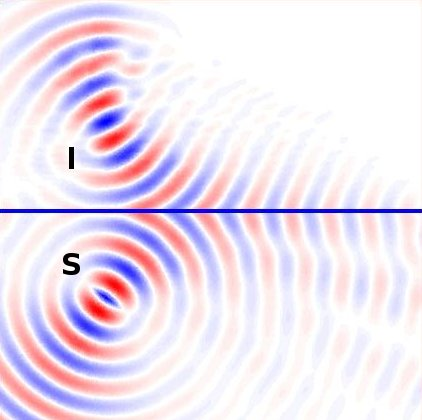
\includegraphics[height=6cm]{pics/nim_lens}
  \end{center}
  \caption{Negative refraction and perfect lens effect. The lower half
    plane is a PIM and the upper half plane is a NIM, with the same
    absolute value of the refractive index. Perfect self focusing is
    achieved. ``S'' stands for ``Source'', ``I'' for ``Image''.}
  \label{fig:nim_lens}
\end{figure}

\OKKIO{NIM e' sempre dispersivo: kramers konig}

The simulation has been carried out with a dispersive version of our
algorithm. Kramers-Konig relations impose that a negative index
material must be dispersive in order to not violate causality
\cite{jackson_classical}. Besides, even if only monofrequency sources
are present in the simulation, naively setting negative $\epsilon$
and $\mu$ to the algorithm makes it unstable. A fully dispersive
algorithm must be employed.

\OKKIO{FDTD dispersive: drude medium -- taflove}

We have implemented dispersive materials for the 2-D time domain
algorithm, with baricentric dual grids. The model chosen is the one
described in \cite{taflove_computational} of Drude media.

\OKKIO{articolo}

The algorithm has been empoyed to study more in detail the negative
refraction phenomenon, with particular attention to a time-limited,
i.e. broadband, input field. Each frequency in the input spectrum will
see a different refractive index for the NIM, due to its dispersive
nature, some will be negativly refracted, some positively and some
totally reflected.

In \cite{bolla_energy} conclusions are drawn. \OKKIO{dilungarsi?}

